% This is text associated with the open textbook "Open Electromagnetics"
% See immediately below for author, date
% This work is licensed under the Creative Commons Attribution-ShareAlike 4.0 International License. (CC BY-SA 4.0) 
% To view a copy of the license, visit http://creativecommons.org/licenses/by-sa/4.0/

%ORB TITLE Ampere's Circuital Law (Magnetostatics): Integral Form
%ORB AUTHOR 0        # S.W. Ellingson, Virginia Tech (ellingson@vt.edu)
%ORB DATE 20180806   # yyyymmdd
%ORB ABSTRACT Ampere's Circuital Law (Magnetostatics): Integral Form

\label{m0019_Amperes_Law_Magnetostatics} % <-- Must match name of this file and module directory name.  Don't mess with this!
\index{Ampere's law!magnetostatics|(}

Ampere's circuital law (ACL) relates current to the magnetic field associated with the current.
In the magnetostatic regime, the law is (see also Figure~\ref{m0019_fACL}):
%
\begin{equation}   
\boxed{
\oint_{\mathcal C}{ {\bf H} \cdot d{\bf l} } = I_{encl}  
}
\label{m0019_eACL}
\end{equation}
%
That is, the integral of the magnetic field intensity ${\bf H}$ over a closed path ${\mathcal C}$ is equal to the current enclosed by that path, $I_{encl}$.
Before proceeding to interpret this law, it is useful to see that it is dimensionally correct. 
That is, ${\bf H}$ (units of A/m) integrated over a distance (units of m) yields a quantity with units of current (i.e., A).
%
\begin{figure}[b!]
\begin{center}
\pdftooltip{{  % note double braces
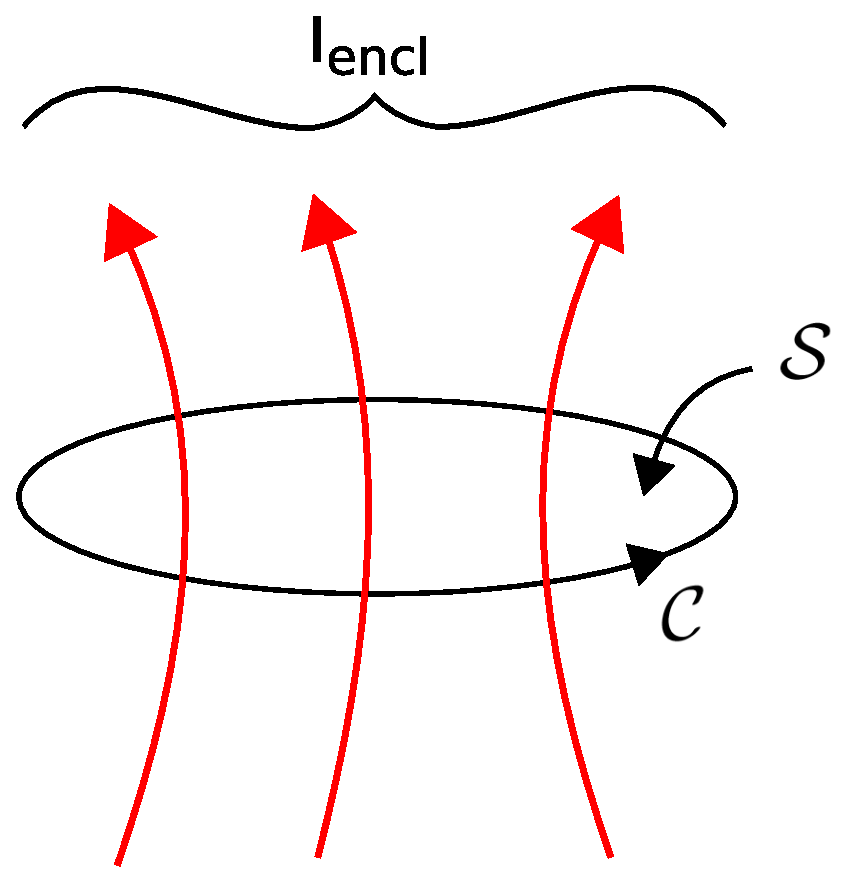
\includegraphics[width=1.5in]{modules/m0019_fACL.eps}
% https://commons.wikimedia.org/wiki/File:M0019_fACL.svg
}}{The figure shows a circle, with surface S and path C. On the path, C, is an arrow that points to the right to indicate counter-clockwise direction. Through the circle are three vectors, the left two bent slightly to the left and the right one bent slightly to the right. All three vectors are labeled "I sub encl".}
\end{center} 
\centerline{\scriptsize 
\copyright~\hyperref[m0019_fACL_Credit]{K.\ Kikkeri} 
\href{https://creativecommons.org/licenses/by-sa/4.0/}{CC BY~SA 4.0} 
} 
\caption{
\label{m0019_fACL}
Reference directions for Ampere's Circuital Law (Equation~\ref{m0019_eACL}).
}
\end{figure}    

In general, $I_{encl}$ may be either positive or negative.
The direction corresponding to positive current flow must be correctly associated with ${\mathcal C}$.
The relationship follows the \emph{right-hand rule} of Stokes' Theorem (Section~\ref{m0051_Stokes_Theorem}) summarized as follows.  The direction of positive $I_{encl}$ is the direction in which the fingers of the right hand intersect any surface ${\mathcal S}$ bordered by ${\mathcal C}$ when the thumb of the right hand points in the direction of integration. The connection to Stokes' Theorem is not a coincidence. See Section~\ref{m0118_Amperes_Law_Magnetostatics_Integral-to-Differential} for more about this.

Note that ${\mathcal S}$ can be \emph{any} surface that is bounded by ${\mathcal C}$ -- not just the taut surface implied in Figure~\ref{m0019_fACL}.

%ORB HIGHLIGHT
\begin{mdframed}[backgroundcolor=yellow!20,nobreak=true] 
The integral form of Ampere's Circuital Law for magnetostatics (Equation~\ref{m0019_eACL}) relates the magnetic field along a closed path to the total current flowing through any surface bounded by that path.
\end{mdframed}

ACL plays a role in magnetostatics that is very similar to the role played by the integral form of Gauss' Law in electrostatics (Section~\ref{m0014_Gauss_Law_Integral_Form}). 
That is, ACL provides a means calculate the magnetic field given the source current.
ACL also has a similar limitation.  Generally, symmetry is required to simplify the problem sufficiently so that the integral equation may be solved.
Fortunately, a number of important problems fall in this category.
Examples include the problems addressed in
Sections~\ref{m0119_Magnetic_Field_of_a_Long_Wire} (magnetic field of a line current), 
\ref{m0120_Magnetic_Field_of_a_Coil} (magnetic field inside a straight coil), 
\ref{m0049_Magnetic_Field_of_a_Toroidal_Coil} (magnetic field of a toroidal coil), 
\ref{m0121_Magnetic_Field_of_an_Infinite_Current_Sheet} (magnetic field of a current sheet), and 
\ref{m0023_Boundary_Conditions_on_H} (boundary conditions on the magnetic field intensity).
For problems in which the necessary symmetry is not available, the differential form of ACL may be required (Section~\ref{m0118_Amperes_Law_Magnetostatics_Integral-to-Differential}).

Finally, be aware that the form of ACL addressed here applies to magnetostatics only.  
In the presence of a \emph{time-varying} electric field, the right side of ACL includes an additional term known as the \emph{displacement current}
\index{displacement current} 
\index{current!displacement|see{displacement current}}
(Section~\ref{m0053_Displacement_Current_Amperes_Law}).

%-------------------------------------------------------

{\bf Additional Reading:}
\begin{itemize}
\item ``\href{https://en.wikipedia.org/wiki/Maxwell's_equations}{Maxwell's Equations}'' on Wikipedia.
\item ``\href{https://en.wikipedia.org/wiki/Ampere's_circuital_law}{Ampere's Circuital Law}'' on Wikipedia.
\end{itemize}

\index{Ampere's law!magnetostatics|)}
